\documentclass{article}
\usepackage{amsmath}
\usepackage{tikz}
\usetikzlibrary{arrows.meta}

\begin{document}

\begin{figure}[h]
    \centering
    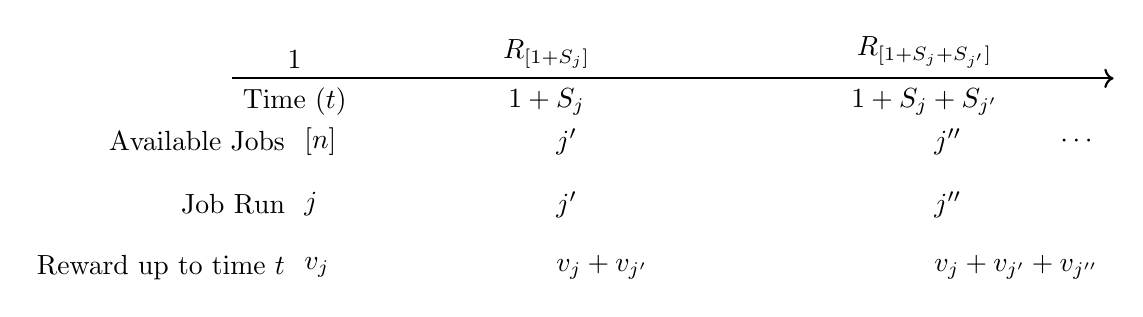
\begin{tikzpicture}[scale=0.8]
        \draw[->, thick] (-2,0) -- (12,0);
        
        \node at (-1,0) [below] {Time ($t$)};
        \node at (-1,0) [above] {$1$};
        \node at (3,0) [below] {$1 + S_j$};
        \node at (3,0) [above] {$R_{[1+S_j]}$};
        \node at (9,0) [below] {$1 + S_j + S_{j'}$};
        \node at (9,0) [above] {$R_{[1+S_j+S_{j'}]}$};
        
        \node at (-1,-1) [left] {Available Jobs};
        \node at (-1,-1) [right] {$[n]$};
        
        \node at (-1,-2) [left] {Job Run};
        \node at (-1,-2) [right] {$j$};
        
        \node at (-1,-3) [left] {Reward up to time $t$};
        \node at (-1,-3) [right] {$v_j$};
        
        \node at (3,-1) [right] {$j'$};
        \node at (3,-2) [right] {$j'$};
        \node at (3,-3) [right] {$v_j + v_{j'}$};
        
        \node at (9,-1) [right] {$j''$};
        \node at (9,-2) [right] {$j''$};
        \node at (9,-3) [right] {$v_j + v_{j'} + v_{j''}$};
        
        \node at (11,-1) [right] {$\cdots$};
    \end{tikzpicture}
    \caption{The figure demonstrates a sample execution according to our model. We select job $j$ at time $t=1$ which gives a value $v_j$, and causes the system to be busy for $S_j$ time units. Once free, we select job $j'$ from the set of available jobs and obtain (additional) value $v_{j'}$, and so on.}
    \label{fig:sample_execution}
\end{figure}

\end{document}